\chapter{DESARROLLO DEL EXPERIMENTO}
En este capítulo se detalla el proceso explicado en el capítulo anterior para cada actividad de la metodología aplicada, así como los entregables comprometidas.

\section{Comprensión del negocio}

\section{Comprensión de los datos}
\textbf{Actividad 1: Construir base de datos de Metainformación}
\\
El punto de partida para la construcción de los conjuntos de datos que se usaron más adelante en cada modelo de acuerdo a su modalidad fue la adquisición de bases de datos capturadas mensualmente desde finales del 2015 hasta 2019 por la página Web Robots (\url{https://webrobots.io/kickstarter-datasets/}), como se aprecia en la Figura \ref{4:fig1}. El sitio ofrece poder descargarlos en archivos de valores separados por comas (.csv) como en formato JSON. Para el presente trabajo, se optó por la primera opción. De acuerdo con \cite{ot_webrobots2019kickstarter}, creadores del sitio Web Robots, se ejecutan robots en dos servidores en la nube encargados de recolectar en un determinado punto del día y una vez al mes información de las campañas que aparecen en Kickstarter.

\begin{figure}[!ht]
	\begin{center}
		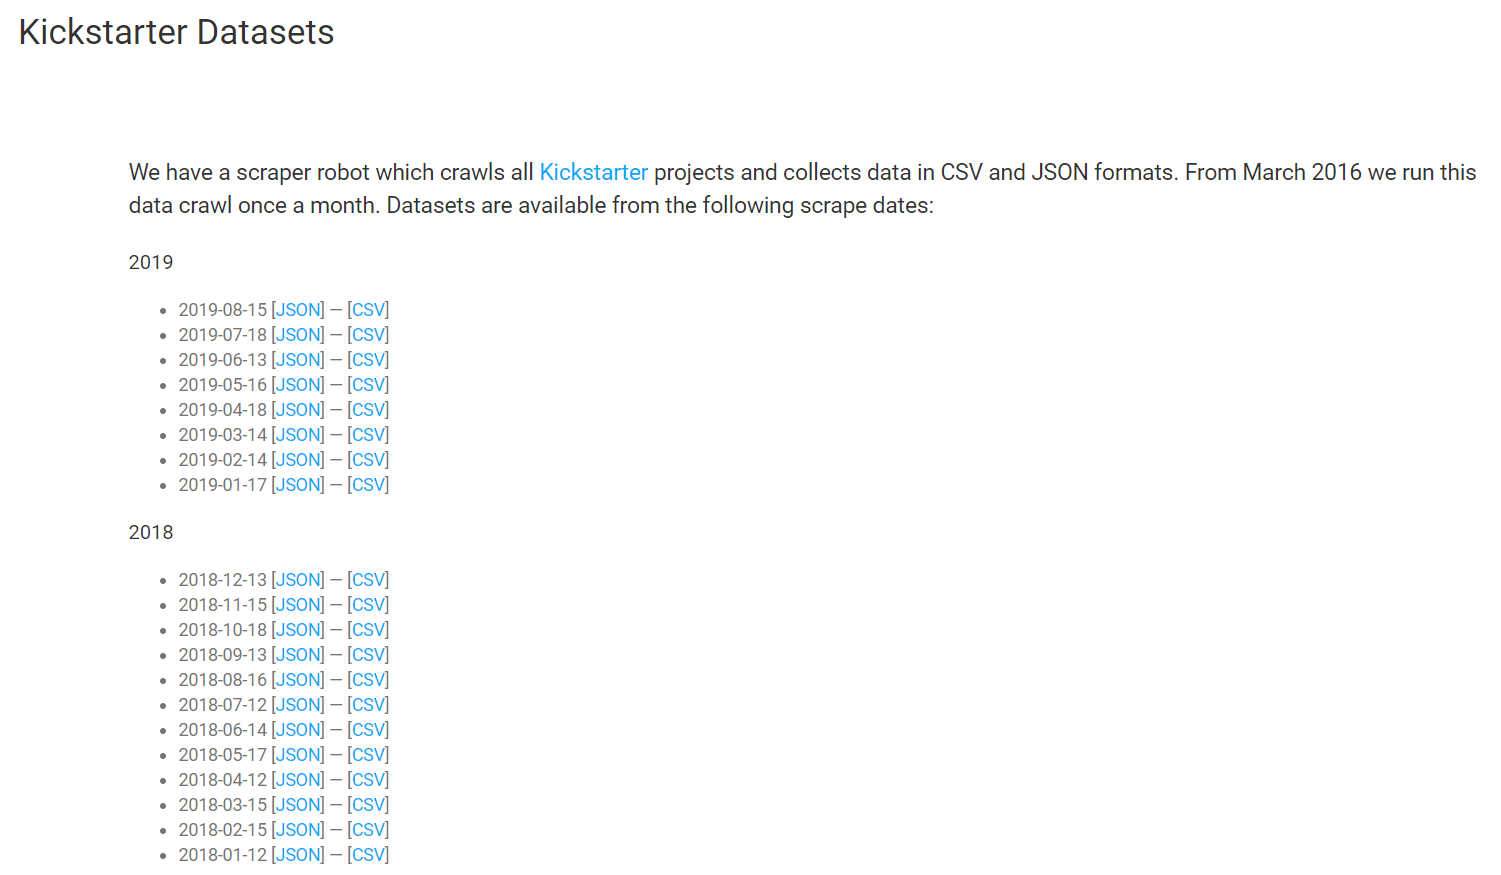
\includegraphics[width=1\textwidth]{4/figures/web_robots_2019.png}
		\caption[Vista del website Web Robots (visitado en agosto del 2019)]{Vista del website Web Robots (visitado en agosto del 2019).\\
			Fuente: \cite{ot_webrobots2019kickstarter}}
		\label{4:fig1}
	\end{center}
\end{figure}

A continuación, los archivos descargados que se encontraban fraccionados en varios archivos .csv, donde luego de ser descomprimidos, fueron unidos por mes de captura y almacenados en carpetas independientes por mes, cuyo peso individual osciló entre 1 y 5 gigabytes (GB). Con el fin de ahorrar espacio en la computadora, las partes originales fueron eliminadas.

En la Figura \ref{4:fig2} se detalla el tamaño del conjunto de datos total al corte del periodo de captura de información Julio 2019, aproximadamente más de 212 mil proyectos de todas las categorías y 37 columnas de variables.

\begin{figure}[h]
	\begin{center}
		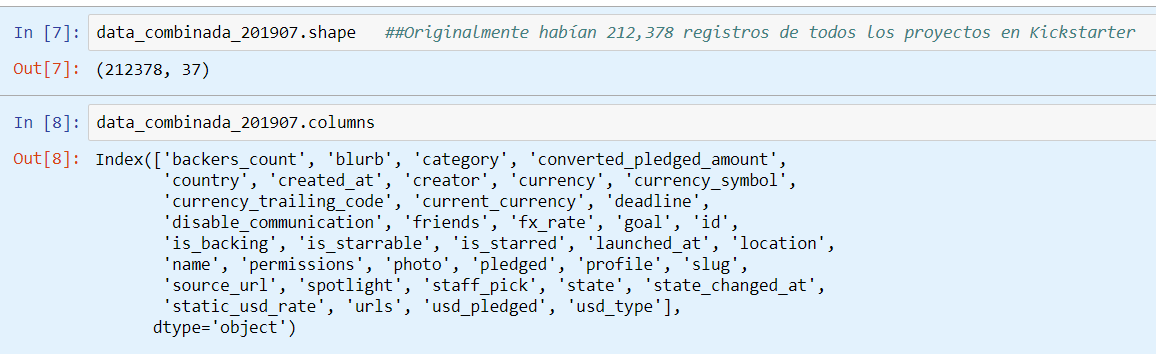
\includegraphics[width=0.9\textwidth]{4/figures/dataset_201907.png}
		\caption[Tamaño de conjunto de datos al corte de Julio 2019]{Tamaño de conjunto de datos al corte de Julio 2019.\\
			Fuente: Elaboración propia.}
		\label{4:fig2}
	\end{center}
\end{figure}

A cada conjunto de datos generado se filtraron los que pertenecen a la categoría \textit{\textbf{Technology}}. Al no contar con la información de la columna \textit{main\_category}, este proceso se logró utilizando la variable \textit{source\_url} seleccionando aquellos registros que contengan la cadena de caracteres “\textbf{https://www.kickstarter.com/discover/categories/technology}”. En la Figura \ref{4:fig3} se aprecia el resultado del conjunto filtrado por categoría Techonlogy al corte de Julio 2019.

\begin{figure}[h]
	\begin{center}
		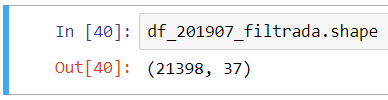
\includegraphics[width=0.5\textwidth]{4/figures/dataset_filtrada_201907.png}
		\caption[Tamaño de conjunto de datos filtrado del corte de Julio 2019]{Tamaño de conjunto de datos filtrado del corte de Julio 2019.\\
			Fuente: Elaboración propia.}
		\label{4:fig3}
	\end{center}
\end{figure}

Cuando se repitió este procedimiento con cada conjunto generado, se observó que la proporción de proyectos tecnológicos en Kickstarter representa el 10\% de la totalidad. Esto se calculó al comparar el tamaño de cada conjunto generado con el total.

A continuación, se unieron los 45 archivos separados por coma (.csv) capturados mensualmente desde noviembre del 2015 hasta agosto del 2019. Se realizaron 2 uniones internamente ya que, a partir de marzo del 2018, algunas de las variables y valores presentan diferente estructura a la de sus predecesoras. Sin embargo, esto no afectó al proceso al cruzar por el nombre de columna.

Luego, se realizó limpieza de datos para las variables \textit{category}, \textit{location}, \textit{photo} y \textit{urls}, y se transformaron las variables numéricas en milisegundos \textit{created\_at}, \textit{launched\_at} y \textit{deadline} a variables de fecha. Esto último permitió calcular la variable \textit{duration} para determinar la duración de la campaña (en días) de un proyecto calculando la diferencia entre la fecha de culminación (\textit{deadline}) y la fecha de lanzamiento (\textit{launched\_at}). Luego se excluyeron los proyectos en proceso de la variable \textit{state} para conservar los culminados, es decir, aquellos cuyo valor sea “successful” o “failed” ya que se analizarán solamente los proyectos que han sido exitosos o fracasados. Los proyectos cancelados o suspendidos no aparecieron. El último paso del flujo consistió en generar y exportar el archivo final en formato .csv. En la Figura \ref{4:fig4} se visualiza el conjunto final de Metainformación subido públicamente a la plataforma Kaggle. Cada variable se detalla en la Tabla \ref{4:table1}.

\begin{figure}[h]
	\begin{center}
		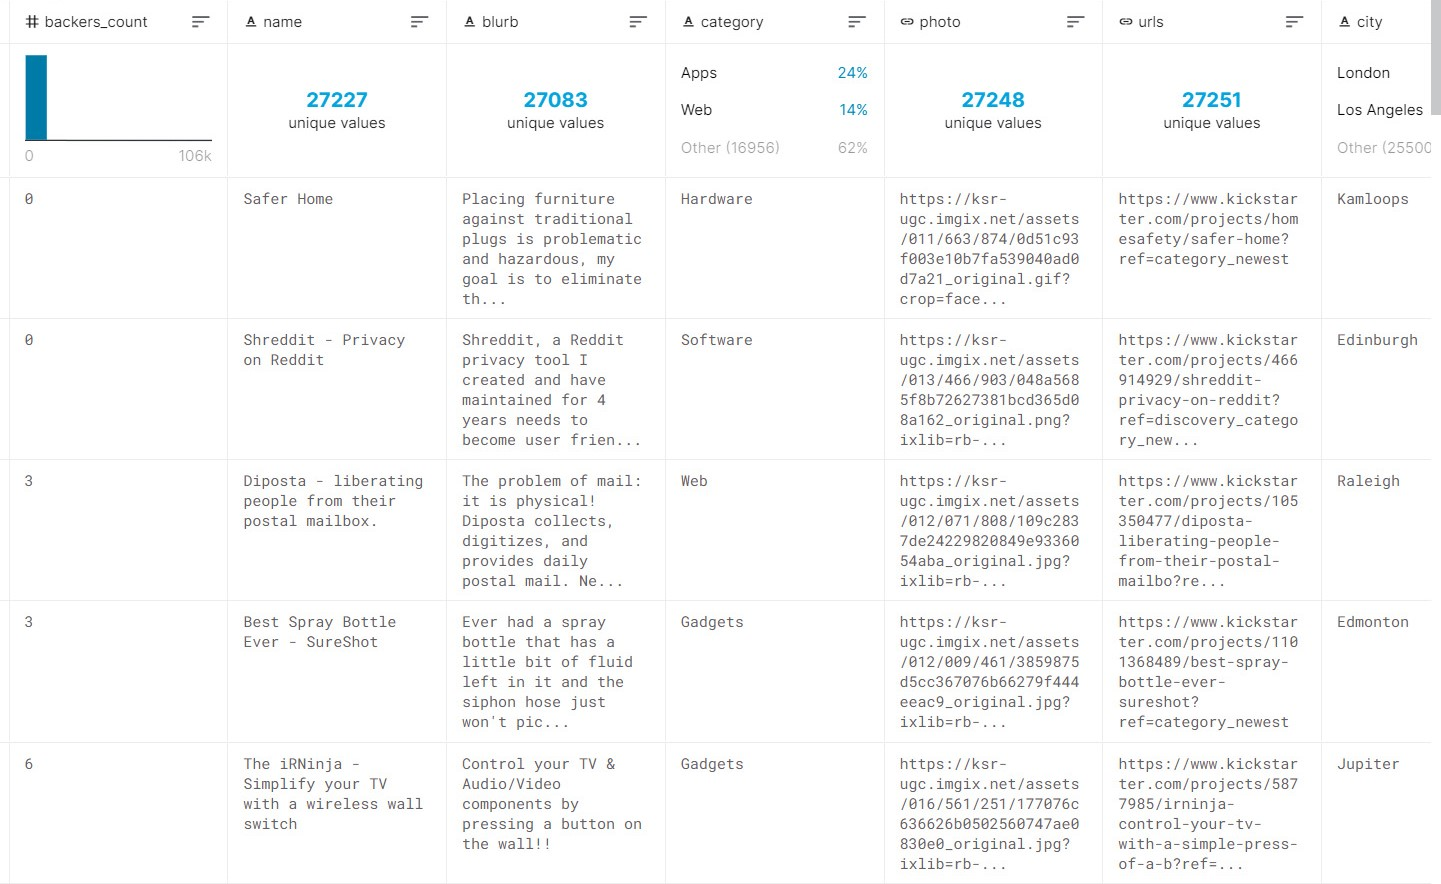
\includegraphics[width=1\textwidth]{4/figures/metadata_kaggle_preview.jpg}
		\caption[Visualización del archivo de metainformación subido a Kaggle]{Visualización del archivo de metainformación subido a Kaggle.\\
			Fuente: Elaboración propia.}
		\label{4:fig4}
	\end{center}
\end{figure}

\begin{table}[h!]
	\caption[Diccionario de datos del dataset final de Metainformación]{Diccionario de datos del dataset final de Metainformación.}
	\label{4:table1}
	\centering
	\small
	\begin{tabular}{ |m{3cm}|m{10cm}|m{2cm}|  }
		\hline
		\Centering \textbf{VARIABLE}& \Centering \textbf{DETALLE}& \Centering \textbf{TIPO DE DATO}\\
		\hline
		\textbf{id} & Identificador del proyecto. & number \\
		\hline
		\textbf{backers\_count} & Número de patrocinadores de la campaña del proyecto. & number \\
		\hline
		\textbf{name} &	Nombre del proyecto. &	string \\
		\hline
		\textbf{blurb} & Propaganda del proyecto. & string \\
		\hline
		\textbf{category} & Categoría (dentro de categoría principal) del proyecto. & string \\
		\hline
		\textbf{photo} & Dirección de enlace de la foto del proyecto. & string \\
		\hline
		\textbf{urls} & Dirección de la página de la campaña del proyecto. & string \\
		\hline
		\textbf{city} & Ciudad del creador del proyecto. & string \\
		\hline
		\textbf{country} & Código de país del creador del proyecto. & string \\
		\hline
		\textbf{goal} &	Monto de la meta de financiamiento del proyecto. &	float \\
		\hline
		\textbf{pledge\_amounts} & Montos disponibles para patrocinar la campaña. & string \\
		\hline
		\textbf{pledged} & Monto final patrocinado de la campaña. & float \\
		\hline
		\textbf{currency} & Divisa del monto final patrocinado. & string \\
		\hline
		\textbf{usd\_pledged} & Monto final patrocinado de la campaña (en USD). & float \\
		\hline
		\textbf{created\_at} & Fecha de creación de la campaña. & date \\
		\hline
		\textbf{launched\_at} & Fecha de lanzamiento de la campaña. & date \\
		\hline
		\textbf{deadline} & Fecha de culminación de la campaña. & date \\
		\hline
		\textbf{duration} &	Duración de la campaña (en días). &	number \\
		\hline
		\textbf{state} & Estado de financiamiento del proyecto. & string \\
		\hline
	\end{tabular}
	\par	%%Salto de linea
	\bigskip
	\begin{flushleft}	%%Alinear a la izquierda sin justificar
		\small Fuente: Elaboración propia.
	\end{flushleft}
\end{table}

\textbf{Actividad 2: Construir base de datos de Descripción}
\\
La variable \textit{description} se obtuvo utilizando web scraping en cada proyecto gracias a la variable \textit{urls}. Para ello, y como se describe en la Figura \ref{4:fig5}, se elaboró un algoritmo usando la librería BeautifulSoup que, mediante la navegación al contenido de estas páginas a través de un agente falso, se dirigió a las descripciones de los proyectos identificando las etiquetas con clase llamada “\textbf{rte\_\_content js-full-description responsive-media}” y las almacenó en un vector vacío, uniendo previamente los párrafos y eliminando caracteres especiales, para posteriormente asignarle la id correspondiente y guardarlo en un archivo de extensión .csv. En caso el algoritmo no encuentre esta clase dentro de las páginas (IndexError), el vector almacenaba un registro nulo.

\begin{figure}[!ht]
	\begin{center}
		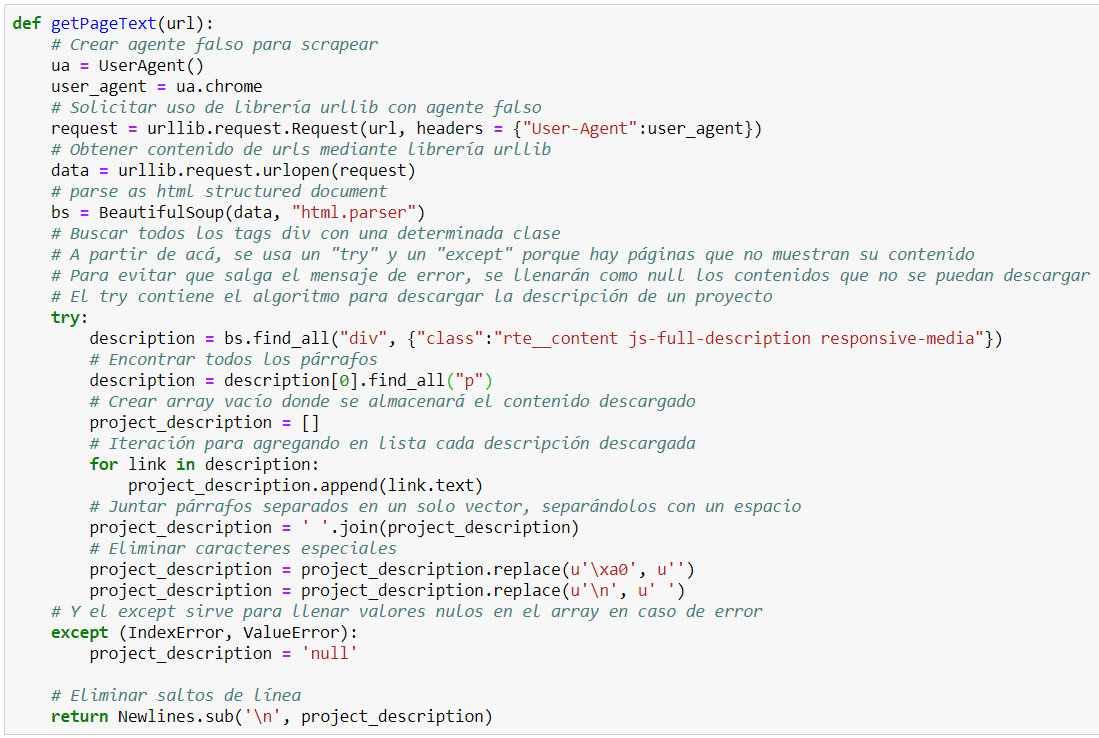
\includegraphics[width=0.8\textwidth]{4/figures/description_scraping.png}
		\caption[Función del algoritmo web scraping de la descripción de proyectos]{Función del algoritmo web scraping de la descripción de proyectos.\\
			Fuente: Elaboración propia.}
		\label{4:fig5}
	\end{center}
\end{figure}

Debido a la gran cantidad de memoria y tiempo que iba a presentar este proceso, se determinó fraccionar los 27,251 proyectos en tres partes y repetir el mismo en cada uno de ellos. El tiempo aproximado de descarga de cada fracción fue de 6 horas.

Finalmente, las tres partes fueron unidas, se reemplazaron los valores nulos por espacios en blanco y se guardó como un nuevo archivo de valores separados por coma (.csv) en código Unicode UTF-8 para la lectura de caracteres no alfabéticos.

El archivo generado fue subido a la plataforma Kaggle de manera pública (Figura \ref{4:fig6}) para que pueda ser descargada a través del API de la web.

\begin{figure}[!ht]
	\begin{center}
		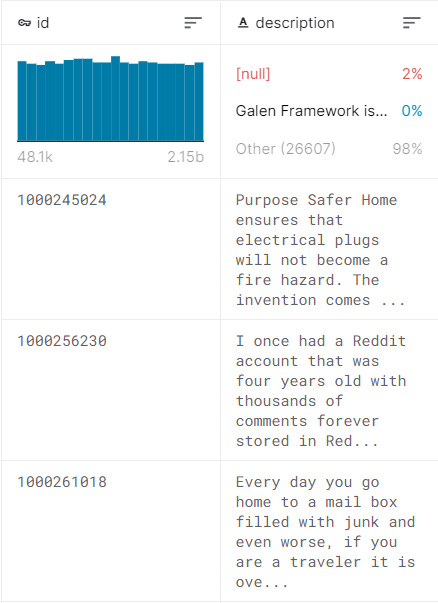
\includegraphics[width=0.4\textwidth]{4/figures/description_kaggle_preview.jpg}
		\caption[Visualización del archivo de descripción subido a Kaggle]{Visualización del archivo de descripción subido a Kaggle.\\
			Fuente: Elaboración propia.}
		\label{4:fig6}
	\end{center}
\end{figure}

\textbf{Actividad 3: Construir base de datos de Comentarios}
\\
Al igual que la descripción, los comentarios se obtuvieron utilizando la variable \textit{urls} para web scraping, pero reemplazando caracteres que contengan desde “\textbf{?ref=}” en adelante, por “\textbf{/comments}” para redireccionarse a la sección de comentarios de cada proyecto.

Los comentarios, al ser dinámicos, no podían extraerse mediante la librería BeautifulSoup como en el caso de las descripciones, por lo que se utilizó la librería Selenium para extraerlos al iniciar una sesión desde Google Chrome, como se observa en el algoritmo de la Figura \ref{4:fig7}.

\begin{figure}[!ht]
	\begin{center}
		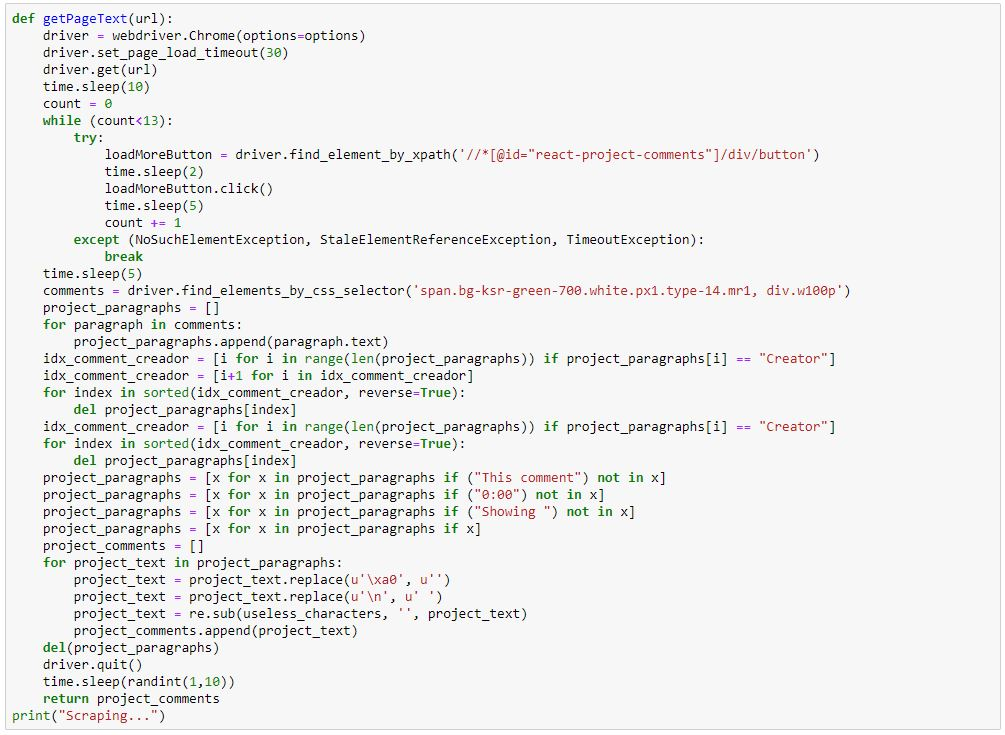
\includegraphics[width=0.8\textwidth]{4/figures/comments_scraping.jpg}
		\caption[Función del algoritmo web scraping de los comentarios]{Función del algoritmo web scraping de los comentarios.\\
			Fuente: Elaboración propia.}
		\label{4:fig7}
	\end{center}
\end{figure}

La función consiste en redireccionarse a la sección de comentarios del proyecto, esperar un máximo de 30 segundos de carga de la página, hacer clic en el botón “Load More” (Cargar más) hasta un límite de no más de 13 veces y almacenar en un vector cada comentario que no pertenezca al creador (se puede diferenciar gracias a una etiqueta en el extremo superior derecho del recuadro del comentario) de manera independiente. El siguiente paso implica la eliminación de ciertos caracteres especiales, emojis y comentarios completos de un patrocinador que no se encuentren en inglés. Finalmente, estos registros de vectores de comentarios con el id del proyecto correspondiente se almacenaron en un archivo .csv por cada fila terminada, el cual se encuentra disponible públicamente en Kaggle (Figura \ref{4:fig8}) así como los anteriores conjuntos comentados para poder ser descargados.

\begin{figure}[!ht]
	\begin{center}
		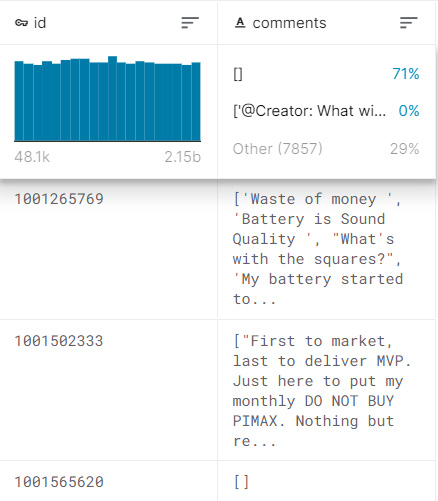
\includegraphics[width=0.4\textwidth]{4/figures/comments_kaggle_preview.jpg}
		\caption[Visualización del archivo de comentarios subido a Kaggle]{Visualización del archivo de comentarios subido a Kaggle.\\
			Fuente: Elaboración propia.}
		\label{4:fig8}
	\end{center}
\end{figure}

Para optimizar la descarga, se crearon 8 instancias en Google Cloud (Figura \ref{4:fig10}), en donde cada una contenía dos copias del algoritmo, con la cantidad de proyectos fraccionada en 16 partes para que sean ejecutados en paralelo. Si bien el tiempo total de la consolidación de esta base de información duró aproximadamente un mes debido a percances de la conexión interna de las instancias y algunos problemas de ineficiencia de la primera versión del algoritmo, durante el transcurso dentro de este lapso de tiempo fueron solucionados hasta lograr optimizar el algoritmo de web scraping y tener el conjunto final de datos tomó menos de 48 horas.

\begin{figure}[!ht]
	\begin{center}
		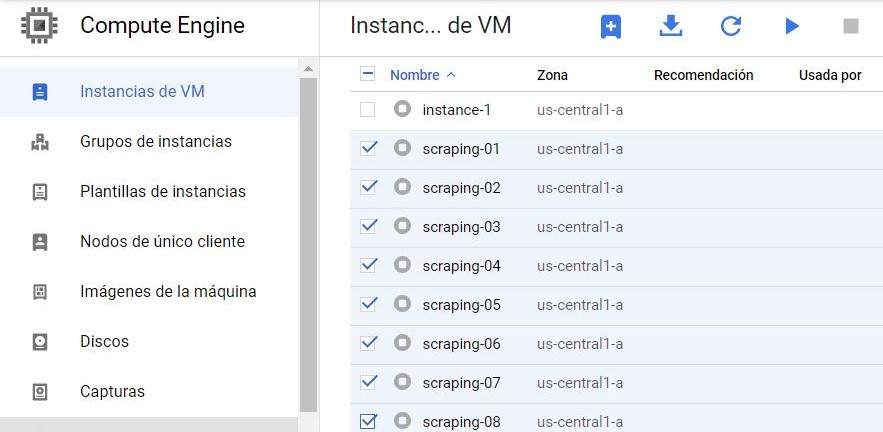
\includegraphics[width=0.7\textwidth]{4/figures/gc_instances_comments.jpg}
		\caption[Instancias lanzadas en paralelo para la extracción de comentarios]{Instancias lanzadas en paralelo para la extracción de comentarios.\\
			Fuente: Elaboración propia.}
		\label{4:fig9}
	\end{center}
\end{figure}

\textbf{Actividad 4: Realizar análisis exploratorio y estadístico de variables considerados}
\\
En esta sección, se analizaron las variables de cada modalidad. Según su estado de financiamiento, los 27,251 proyectos se distribuyen mediante el gráfico de pie de la Figura \ref{4:fig10}. De esta, se observa que más del 70\% de estos fracasaron.

\begin{figure}[!ht]
	\begin{center}
		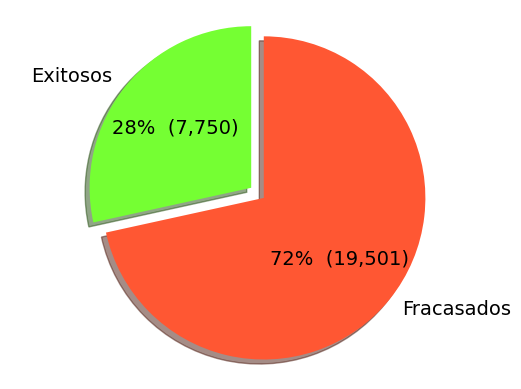
\includegraphics[width=0.55\textwidth]{4/figures/projects by state.png}
		\caption[Distribución de proyectos tecnológicos según su estado]{Distribución de proyectos tecnológicos según su estado.\\
			Fuente: Elaboración propia.}
		\label{4:fig10}
	\end{center}
\end{figure}

Al visualizarlos por año (Figura \ref{4:fig11}), se puede ver que el histórico comprende entre los periodos 2009 y 2019, siendo la gran mayoría perteneciente al año 2015.

\begin{figure}[!ht]
	\begin{center}
		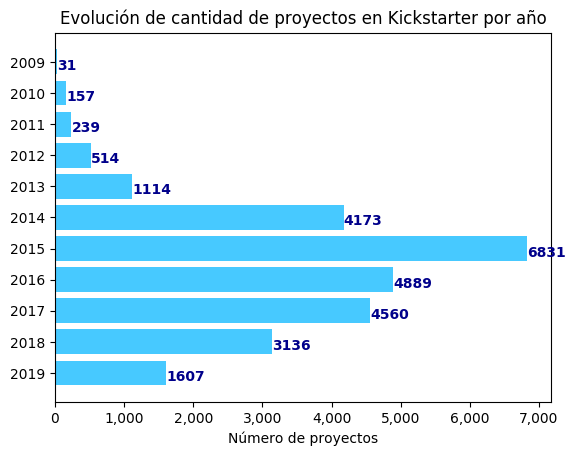
\includegraphics[width=0.7\textwidth]{4/figures/projects state by year.png}
		\caption[Evolución de cantidad de proyectos tecnológicos por año]{Evolución de cantidad de proyectos tecnológicos por año.\\
			Fuente: Elaboración propia.}
		\label{4:fig11}
	\end{center}
\end{figure}

La evolución histórica detallada por su estado se observa en la Figura \ref{4:fig12}.

\begin{figure}[!ht]
	\begin{center}
		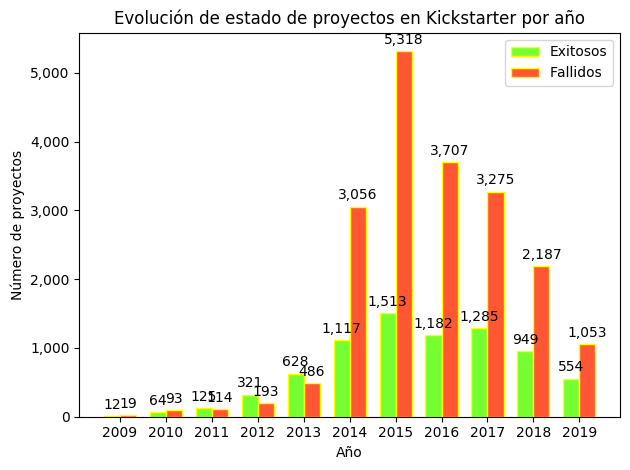
\includegraphics[width=0.7\textwidth]{4/figures/projects state evolution by year.png}
		\caption[Evolución de proyectos tecnológicos, por su estado y año]{Evolución de proyectos tecnológicos, por su estado y año.\\
			Fuente: Elaboración propia.}
		\label{4:fig12}
	\end{center}
\end{figure}

Por el lado de la modalidad Metainformación, de las 19 variables de la Tabla \ref{4:table1}, se consideraron como potenciales variables independientes a 5 numéricas (\textit{backers\_count}, \textit{goal}, \textit{pledged}, \textit{usd\_pledged} y \textit{duration}), 3 categóricas (\textit{category}, \textit{country} y \textit{currency}) y 1 del tipo lista compuesta por números (\textit{pledge\_amounts}).

Para las variables categóricas, se realizaron gráficos de pastel para observar la distribución de sus valores. Así tenemos la Figura \ref{4:fig13} para las categorías de tecnología, Figura \ref{4:fig14} para los países (por código) y la Figura \ref{4:fig15} para las divisas del monto final patrocinado (por código). De estos tres gráficos, se observa que más de la mitad de patrocinadores provienen de los Estados Unidos (US) e invierten en dólares (USD). El segundo y tercer lugar los constituyen personas de Gran Bretaña (GB) y Canadá (CA), invirtiendo en sus monedas locales respectivas (GBP y CAD). Por el lado de las categorías, la más recurrente son de Apps, representando casi la cuarta parte del universo observado.

\begin{figure}[htbp]
	\begin{center}
		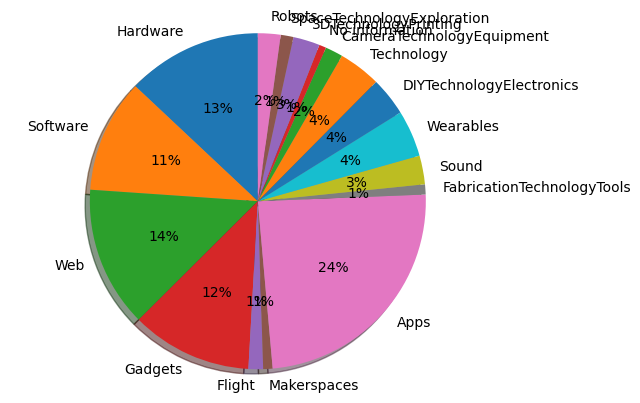
\includegraphics[width=0.65\textwidth]{4/figures/category_distribution.png}
		\caption[Distribución de categorías de tecnología]{Distribución de categorías de tecnología.\\
			Fuente: Elaboración propia.}
		\label{4:fig13}
		
		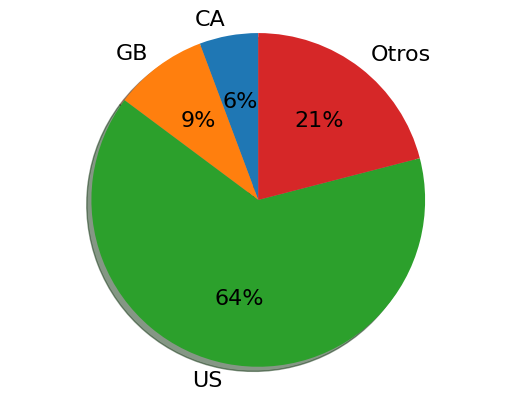
\includegraphics[width=0.53\textwidth]{4/figures/country_distribution.png}
		\caption[Distribución de países]{Distribución de países.\\
			Fuente: Elaboración propia.}
		\label{4:fig14}
		
		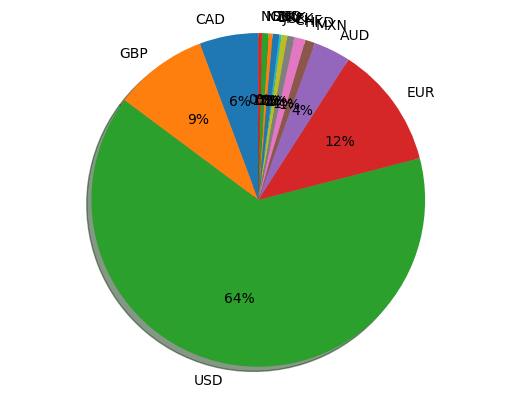
\includegraphics[width=0.53\textwidth]{4/figures/currency_distribution.png}
		\caption[Distribución de divisa del monto patrocinado]{Distribución de divisa del monto patrocinado.\\
			Fuente: Elaboración propia}
		\label{4:fig15}
	\end{center}
\end{figure}

Para las variables numéricas, se calcularon sus datos estadísticos con ayuda de diagramas de caja y bigote:
\begin{itemize}
	\item Número de patrocinadores de la campaña (\textit{backers\_count}):
	\begin{itemize}
		\item Rango de valores: [0; 105,857]
		\item Media: 208.710469340575
		\item Mediana: 9.487
		\item Desviación estándar: 1,179.68237749203
		\item Varianza: 1,391,650.51176525
		\begin{figure}[!ht]
			\begin{center}
				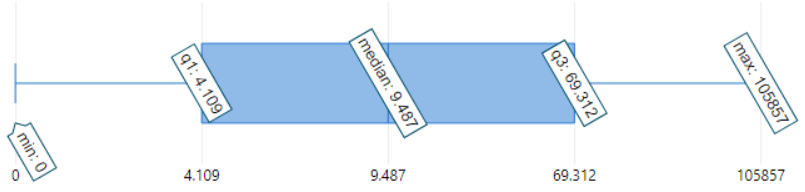
\includegraphics[width=0.7\textwidth]{4/figures/caja_bigote_backers.png}
				\caption[Diagrama de caja y bigote de patrocinadores]{Diagrama de caja y bigote de patrocinadores.\\
					Fuente: Elaboración propia.}
				\label{4:fig16}
			\end{center}
		\end{figure}
	\end{itemize}
	\item Monto meta de la campaña (\textit{goal}):
	\begin{itemize}
		\item Rango de valores: [1; 100,000,000]
		\item Media: 91,263.9666162825
		\item Mediana: 15,762.614
		\item Desviación estándar: 1,259,282.1587922
		\item Varianza: 1,585,791,555,452.35
		\begin{figure}[!ht]
			\begin{center}
				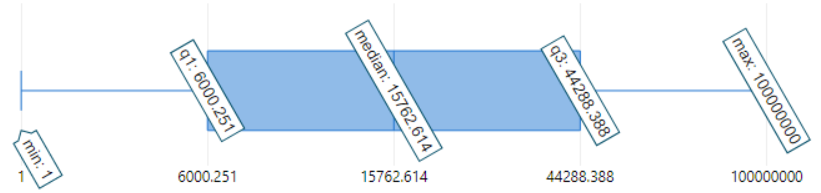
\includegraphics[width=0.7\textwidth]{4/figures/caja_bigote_goal.png}
				\caption[Diagrama de caja y bigote de meta]{Diagrama de caja y bigote de meta.\\
					Fuente: Elaboración propia.}
				\label{4:fig17}
			\end{center}
		\end{figure}
	\end{itemize}
	\item Monto patrocinado al final de la campaña (\textit{pledged}):
	\begin{itemize}
		\item Rango de valores: [0; 17,406,300]
		\item Media: 34,668.5134710787
		\item Mediana: 1,382.933
		\item Desviación estándar: 226,763.900313481
		\item Varianza: 51,421,866,485.3822
		\begin{figure}[!ht]
			\begin{center}
				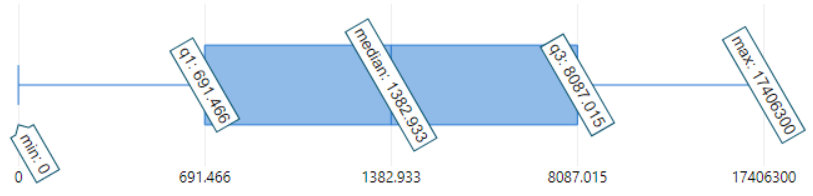
\includegraphics[width=0.7\textwidth]{4/figures/caja_bigote_pledged.png}
				\caption[Diagrama de caja y bigote de monto patrocinado]{Diagrama de caja y bigote de monto patrocinado.\\
					Fuente: Elaboración propia.}
				\label{4:fig18}
			\end{center}
		\end{figure}
	\end{itemize}
	\item Duración de la campaña (\textit{duration}).
	\begin{itemize}
		\item Rango de valores: [1; 92]
		\item Media: 35.4654141132436
		\item Mediana: 30
		\item Desviación estándar: 11.84570862999998
		\item Varianza: 140.320812946853
		\begin{figure}[!ht]
			\begin{center}
				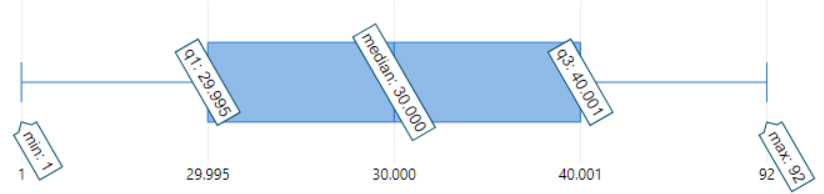
\includegraphics[width=0.7\textwidth]{4/figures/caja_bigote_duration.png}
				\caption[Diagrama de caja y bigote de duración]{Diagrama de caja y bigote de duración.\\
					Fuente: Elaboración propia.}
				\label{4:fig19}
			\end{center}
		\end{figure}
	\end{itemize}
\end{itemize}

Posterior a este entendimiento de datos, se elaboró una matriz de correlaciones (Figura \ref{4:fig20}) para encontrar correlaciones entre ellas y determinar la existencia de alguna variable redundante y descartarla para no afectar el rendimiento del modelo.

\begin{figure}[!ht]
	\begin{center}
		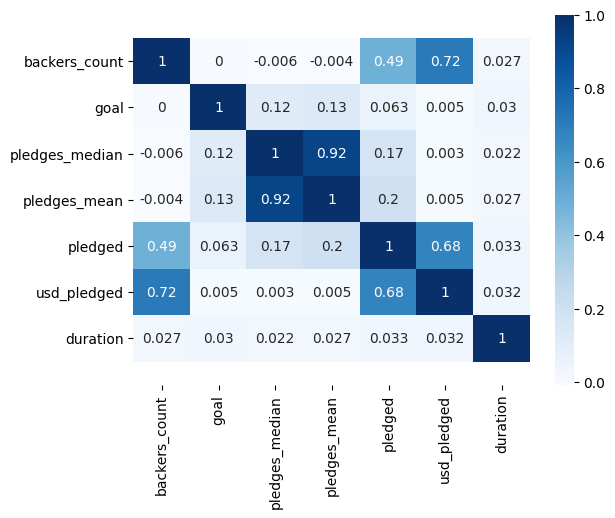
\includegraphics[width=0.65\textwidth]{4/figures/metadata correlation.png}
		\caption[Matriz de correlaciones entre variables independientes]{Matriz de correlaciones entre variables independientes.\\
			Fuente: Elaboración propia.}
		\label{4:fig20}
	\end{center}
\end{figure}

Como se puede apreciar en la figura anterior, la variable \textit{usd\_pledged} está altamente correlacionada con las variables \textit{backers\_count} y \textit{pledged} (ambas con un aproximado de 70\%). Esto quiere decir que dicha variable no es significativa porque explicaría de manera muy similar a las otras dos.

Asimismo, si se observan los registros desde una matriz que contiene, además de gráficos de dispersión de las correlaciones, histogramas de las variables independientes como en la Figura \ref{4:fig21}, se confirma y concluye no utilizar las observaciones comentadas.

\begin{figure}[!ht]
	\begin{center}
		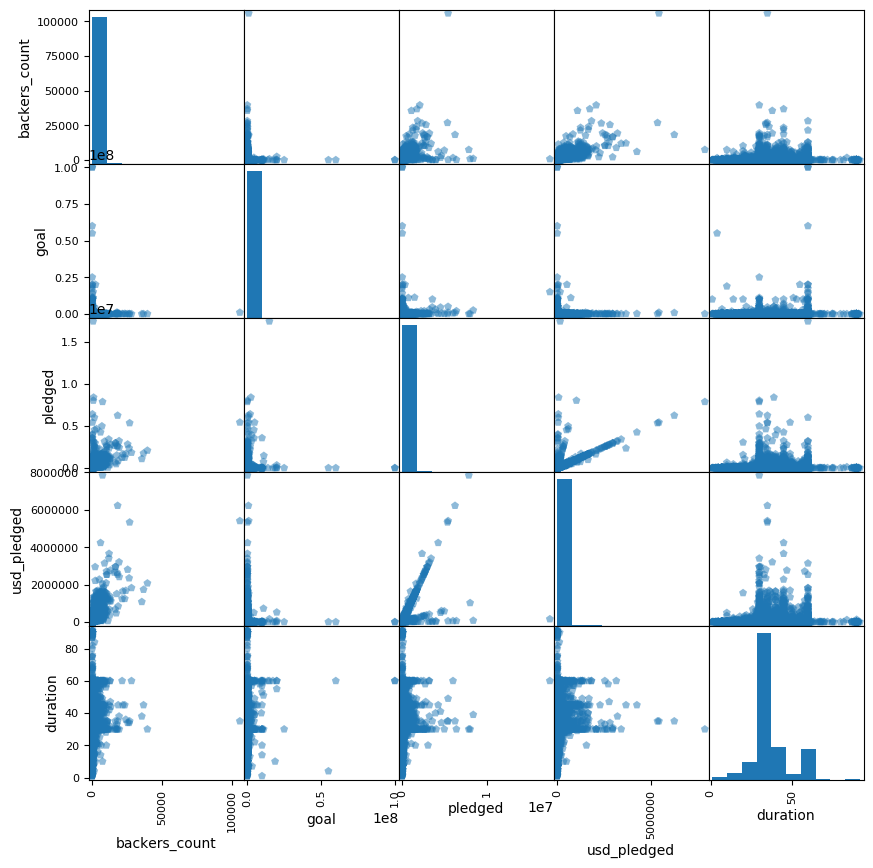
\includegraphics[width=0.80\textwidth]{4/figures/metadata cor-plot1.png}
		\caption[Gráfico de dispersión de correlaciones entre variables independientes]{Gráfico de dispersión de correlaciones entre variables independientes.\\
			Fuente: Elaboración propia.}
		\label{4:fig21}
	\end{center}
\end{figure}

El mismo gráfico, segmentado por las dos clases del estado de financiamiento, se aprecia en la Figura \ref{4:fig22}.

\begin{figure}[!ht]
	\begin{center}
		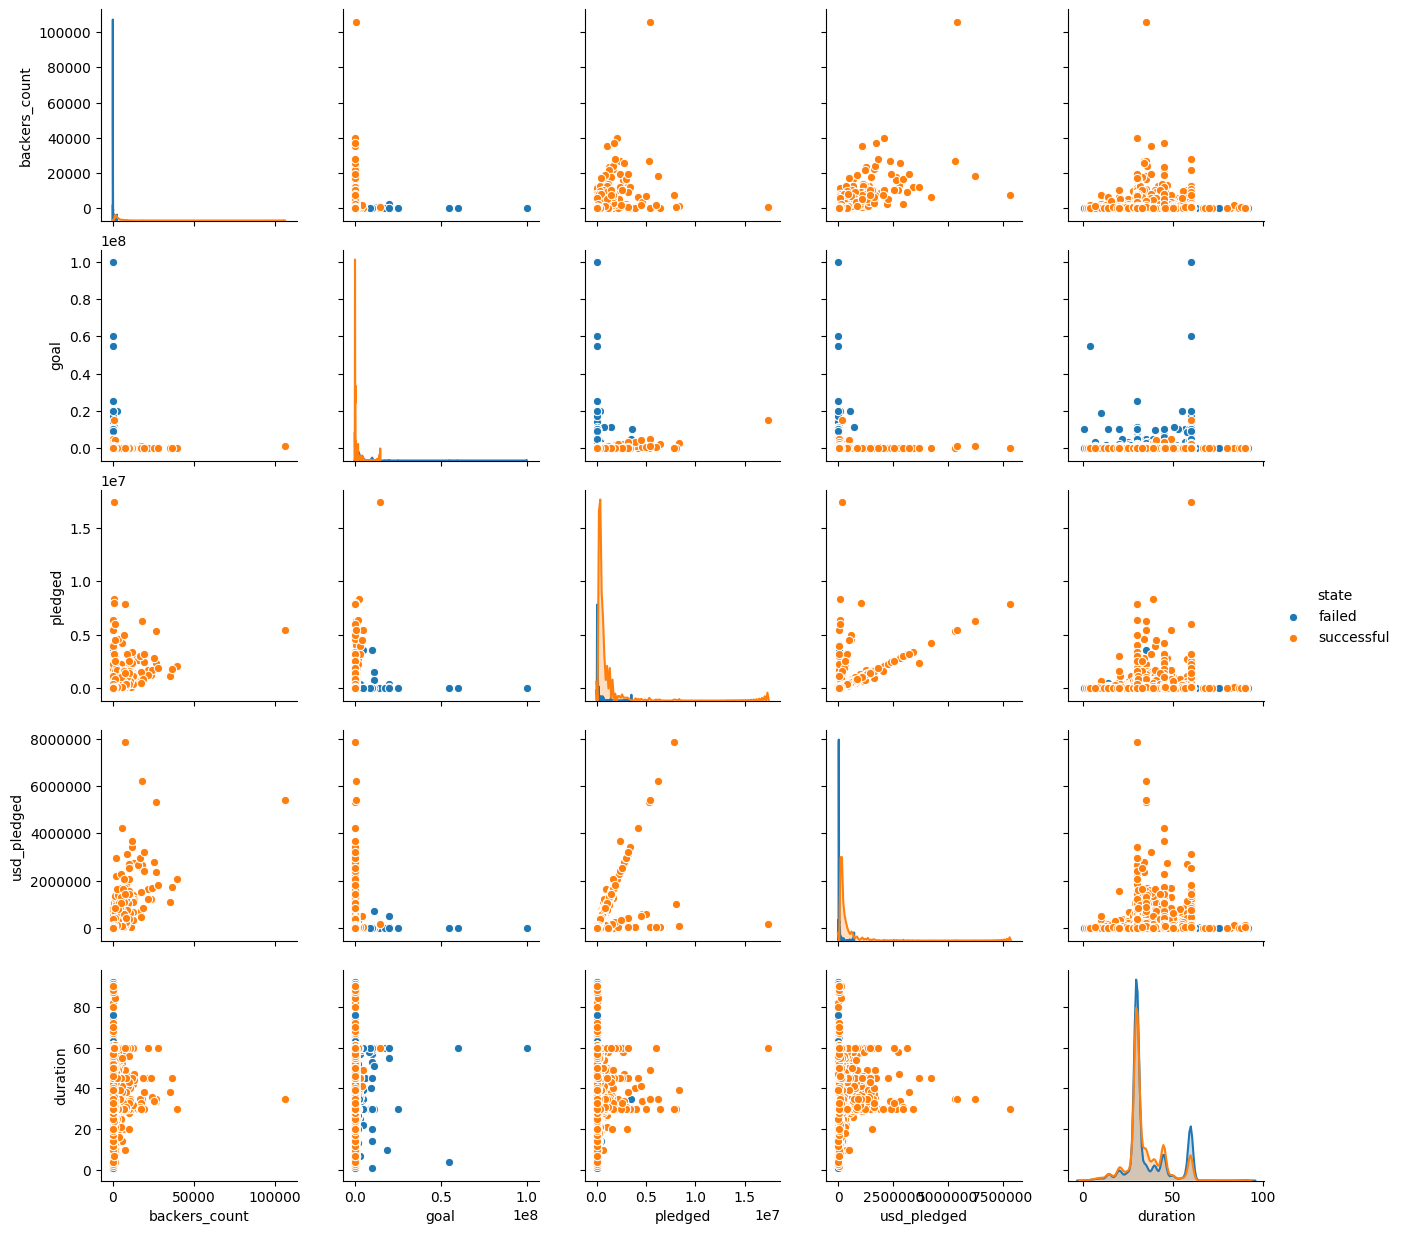
\includegraphics[width=0.80\textwidth]{4/figures/metadata cor-plot2.png}
		\caption[Gráfico alterno de dispersión de correlaciones entre variables independientes]{Gráfico alterno de dispersión de correlaciones entre variables independientes.\\
			Fuente: Elaboración propia.}
		\label{4:fig22}
	\end{center}
\end{figure}

Se concluye entonces que la variable \textit{duration} es la única que sigue una distribución normal.

Por el lado de la modalidad Descripción, solamente 640 proyectos del total (aproximadamente 2\% de la población) no presentaron descripciones por razones externas durante el proceso de extracción de datos en el Web Scraping. De esta cantidad, 512 (80\% de proyectos sin descripciones) no fueron financiados al final de su campaña, es decir, su estado fue fracasado. Mientras que del subconjunto de proyectos con descripciones, casi el 30\% fueron exitosos (Figura \ref{4:fig23}).

\begin{figure}[!ht]
	\begin{center}
		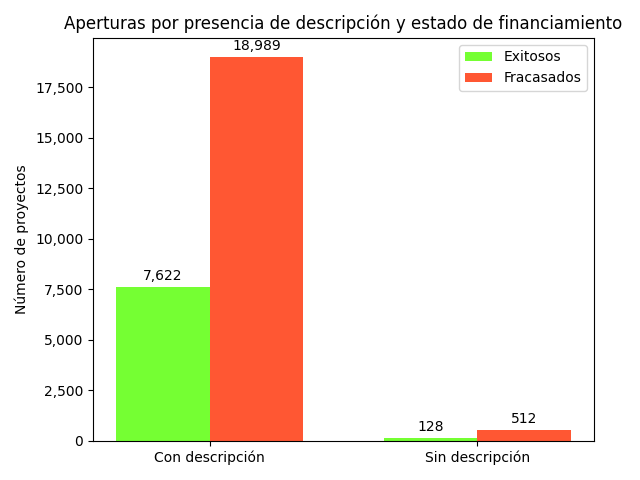
\includegraphics[width=0.7\textwidth]{4/figures/projects description by state.png}
		\caption[Aperturas de proyectos por presencia de comentarios y estado de financiamiento]{Aperturas de proyectos por presencia de comentarios y estado de financiamiento.\\
			Fuente: Elaboración propia.}
		\label{4:fig23}
	\end{center}
\end{figure}

En este universo, el registro con descripción de mayor longitud presentó 5,152 palabras y, a nivel total de proyectos, el vocabulario fue de 165,683 palabras. La Figura \ref{4:fig24} representa la nube de palabras del contenido de cada descripción, donde las más destacadas son aquellas de mayor dimensión.

\begin{figure}[!ht]
	\begin{center}
		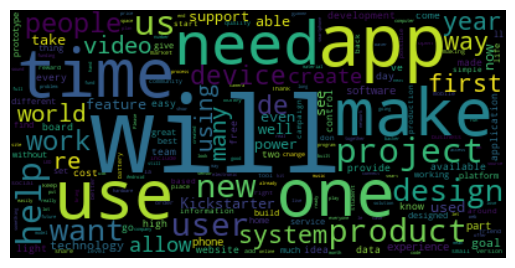
\includegraphics[width=0.7\textwidth]{4/figures/description_wordcloud_original_data.png}
		\caption[Nube de palabras de descripciones]{Nube de palabras de descripciones.\\
			Fuente: Elaboración propia.}
		\label{4:fig24}
	\end{center}
\end{figure}

Finalmente, por el lado de la modalidad Comentarios, al analizar los proyectos exitosos y fracasados de acuerdo a la presencia de comentarios (Figura \ref{4:fig25}), se observa que hay una sólida relación entre aquellos que fracasaron y los que no cuentan con comentarios, mientras que para los proyectos exitosos, la asociación es menos contundente ya que la diferencia entre aquellos que presentan comentarios y los que no es menor.

\begin{figure}[!ht]
	\begin{center}
		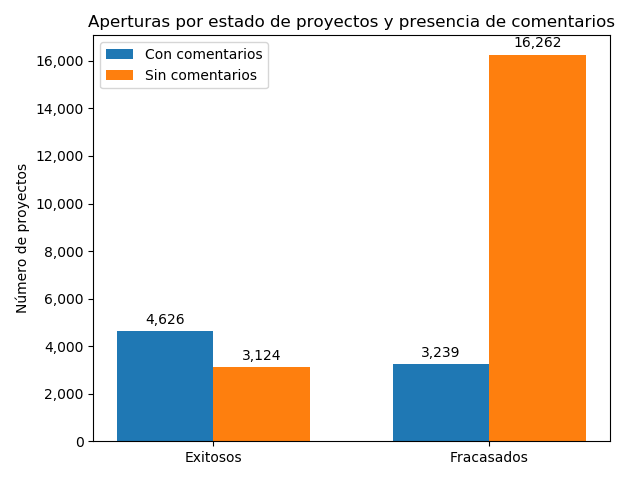
\includegraphics[width=0.7\textwidth]{4/figures/projects state by comment.png}
		\caption[Aperturas de proyectos por estado de financiamiento y presencia de comentarios]{Aperturas de proyectos por estado de financiamiento y presencia de comentarios.\\
			Fuente: Elaboración propia.}
		\label{4:fig25}
	\end{center}
\end{figure}

Ordenando la distribución por presencia de comentarios (Figura \ref{4:fig26}), se observa que del total de los proyectos con comentarios, el 60\% de ellos (4,626 registros) fueron exitosos, encontrándose casi balanceado este subconjunto.

\begin{figure}[!ht]
	\begin{center}
		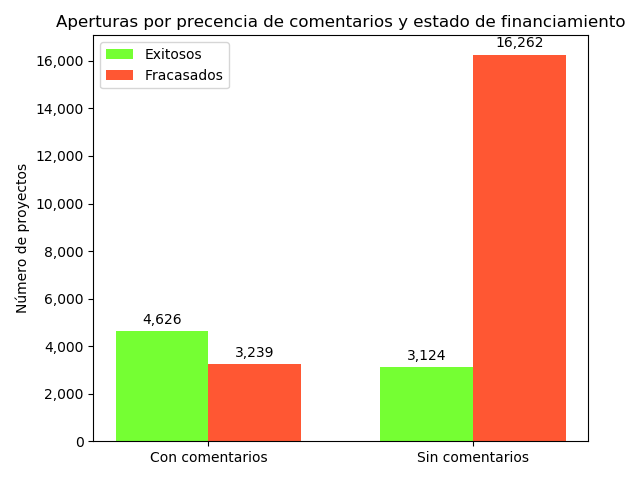
\includegraphics[width=0.7\textwidth]{4/figures/projects comment by state.png}
		\caption[Aperturas de proyectos por presencia de comentarios y estado de financiamiento]{Aperturas de proyectos por presencia de comentarios y estado de financiamiento.\\
			Fuente: Elaboración propia.}
		\label{4:fig26}
	\end{center}
\end{figure}

Asimismo, del universo de proyectos tecnológicos que presentan comentarios, los más de 4 mil proyectos exitosos contienen casi la totalidad de comentarios registrados (97\%), representando más de 475 mil como se aprecia en la Figura \ref{4:fig27}. Estos datos confirma la correlación existe entre la presencia de un volumen considerable de comentarios y su éxito de financiación.

\begin{figure}[!ht]
	\begin{center}
		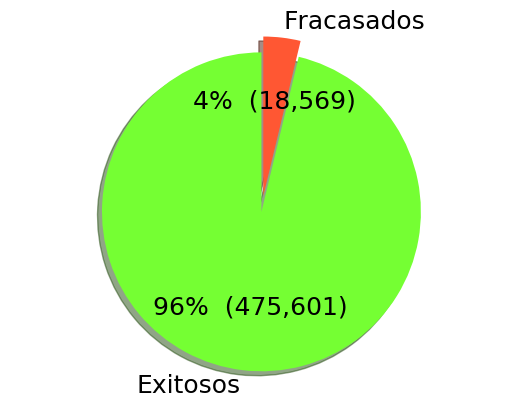
\includegraphics[width=0.75\textwidth]{4/figures/total comments by projects state.png}
		\caption[Distribución de comentarios en proyectos exitosos y fracasados]{Distribución de comentarios en proyectos exitosos y fracasados.\\
			Fuente: Elaboración propia.}
		\label{4:fig27}
	\end{center}
\end{figure}

Respecto al contenido, en la Figura \ref{4:fig28} se ilustra la nube de palabras más frecuentes, respectivamente, luego de quitar URLs, emoticonos y términos en idioma distinto al inglés.

\begin{figure}[htbp]
	\begin{center}
		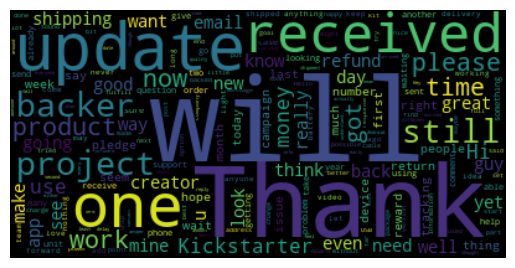
\includegraphics[width=0.68\textwidth]{4/figures/comments_wordcloud_wordunit.png}
		\caption[Nube de palabras de comentarios más frecuentes]{Nube de palabras de comentarios más frecuentes.\\
			Fuente: Elaboración propia.}
		\label{4:fig28}
	\end{center}
\end{figure}

\section{Preparación de los datos}
\textbf{Actividad 1: Pre-procesar base de datos de Metainformación}
\\
De acuerdo a los autores \cite{pr_chen2013kickpredict} (primer antecedente), \cite{pr_chen2015predcrowd} (cuarto antecedente) y \cite{pr_jin2019dayssuccess} (decimotercer antecedente), a las 5 potenciales variables numéricas se adicionaron 7 variables basadas en el mecanismo financiero (mediana (\textit{pledges\_median}), promedio (\textit{pledges\_mean}), valor máximo (\textit{pledges\_max}), valor mínimo (\textit{pledges\_min}), variación estándar (\textit{pledges\_std}) y cantidad de montos disponibles para contribuir (\textit{pledges\_num})) y efecto progresión (porcentaje de financiamiento o completitud (\textit{completeness}) del monto prometido). Esta última se calcula dividiendo el monto alcanzado en el tiempo t, sobre la meta de la campaña, multiplicado por 100\%. La nueva matriz de correlación se observa en la Figura \ref{4:fig29}.

\begin{figure}[!ht]
	\begin{center}
		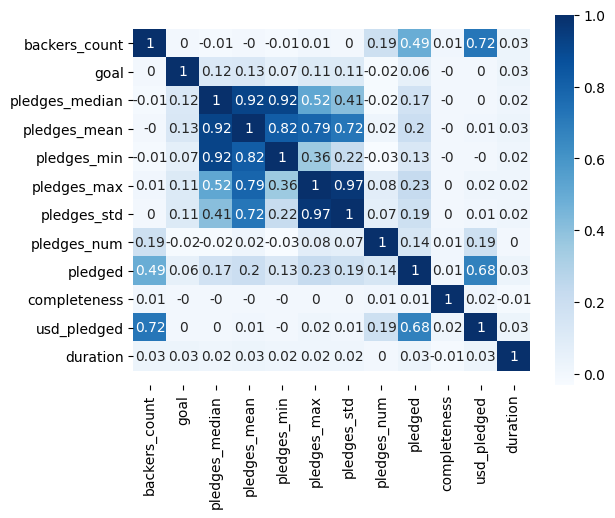
\includegraphics[width=0.85\textwidth]{4/figures/metadata correlation v2.png}
		\caption[Matriz de correlaciones entre variables independientes considerando adicionales]{Matriz de correlaciones entre variables independientes considerando adicionales.\\
			Fuente: Elaboración propia.}
		\label{4:fig29}
	\end{center}
\end{figure}

Para la selección de variables, se consideró a aquellas con correlación clasificada como insignificante, es decir, menor o igual a 0.30 \parencite{tec_mukaka2012correlation}. Las únicas que cumplen son \textit{goal}, \textit{pledges\_num}, \textit{completeness} y \textit{duration}. Sin embargo, algunas de las restantes pueden ser consideradas condicionándose a excluir otras. En la Tabla \ref{4:table2} se listan las 8 combinatorias posibles de variables que se pueden formar.

\begin{table}[h!]
	\caption[Potenciales combinatorias de variables de metainformación]{Potenciales combinatorias de variables de metainformación.}
	\label{4:table2}
	\centering
	\small
	\begin{tabular}{ |m{3.5cm}|m{3.5cm}|m{3.5cm}|m{3.5cm}|  }
		\hline
		%\rowcolor{bluejean}
		\Centering \textbf{Combinación 1}& \Centering \textbf{Combinación 2}& \Centering \textbf{Combinación 3}& \Centering \textbf{Combinación 4}
		\\
		\hline
		\textbf{goal} & \textbf{goal} & \textbf{goal} & \textbf{goal} \\
		\hline
		\textbf{completeness} & \textbf{completeness} & \textbf{completeness} & \textbf{completeness} \\
		\hline
		\textbf{duration} & \textbf{duration} &	\textbf{duration} & \textbf{duration} \\
		\hline
		\textbf{pledges\_num} & \textbf{pledges\_num} & \textbf{pledges\_num} & \textbf{pledges\_num} \\
		\hline
		backers\_count & backers\_count & backers\_count & backers\_count \\
		\hline
		pledges\_median & pledges\_mean & pledges\_min & pledges\_max \\
		\hline
		&  & pledges\_std &  \\
		\hline
		%\rowcolor{turq}
		\multicolumn{4}{c}{ } \\
		\hline
		%\rowcolor{bluejean}
		\Centering \textbf{Combinación 5}& \Centering \textbf{Combinación 6}&
		\Centering \textbf{Combinación 7}& \Centering \textbf{Combinación 8}
		\\
		\hline
		\textbf{goal} & \textbf{goal} & \textbf{goal} & \textbf{goal} \\
		\hline
		\textbf{completeness} & \textbf{completeness} & \textbf{completeness} & \textbf{completeness} \\
		\hline
		\textbf{duration} & \textbf{duration} &	\textbf{duration} & \textbf{duration} \\
		\hline
		\textbf{pledges\_num} & \textbf{pledges\_num} & \textbf{pledges\_num} & \textbf{pledges\_num} \\
		\hline
		pledged & pledged & pledged & pledged \\
		\hline
		pledges\_median & pledges\_mean & pledges\_min & pledges\_max \\
		\hline
		&  & pledges\_std &  \\
		\hline
	\end{tabular}
	\par	%%Salto de linea
	\bigskip
	\begin{flushleft}	%%Alinear a la izquierda sin justificar
		\small Fuente: Elaboración propia.
	\end{flushleft}
\end{table}

\textbf{Actividad 2: Pre-procesar base de datos de Descripción}
\\
Para poder entrenar un modelo de clasificación binaria basado en texto, se debe pre-procesar siguiendo el flujograma de Figura \ref{4:fig30}, que complementa la limpieza de texto referidos previamente (\cite{pr_mitra2014phrases}, segundo antecedente; \cite{pr_yuan2016textanalytics}, séptimo antecedente; y \cite{pr_chen2019keywords_crowdfunding}, decimoquinto antecedente) con el proceso dictado en el curso de Procesamiento de Lenguaje Natural en la Escuela Superior de Economía de la Universidad Nacional de Investigación, Rusia \parencite{tec_zimovnov2018text_preprocessing}. Antes de ejecutar cada paso, los registros de proyectos sin descripciones, es decir, con valor nulo (\textit{NaN}), se convirtieron en cadena (\textit{string}) para evitar problemas de procesamiento de texto. Se remueven las contracciones, caracteres especiales, enlaces externos y contenidos en otros idiomas. Este resultado será tokenizado a palabras individuales con la intención de eliminar palabras de parada en inglés, lematizar las restantes y finalmente juntarlas en una lista, separadas por su proyecto correspondiente.

\begin{figure}[!ht]
	\begin{center}
		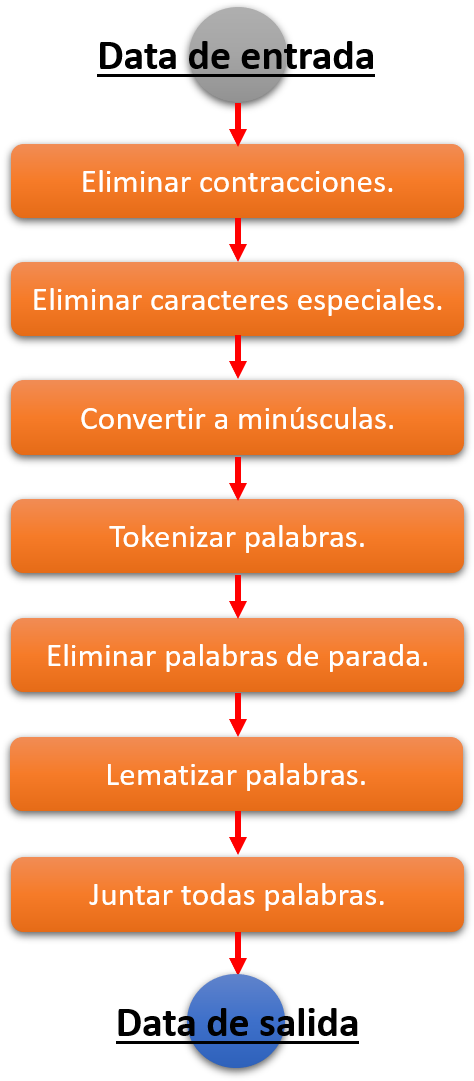
\includegraphics[width=0.35\textwidth]{4/figures/description_data_clean.png}
		\caption[Flujograma de limpieza de conjunto de datos de descripciones]{Flujograma de limpieza de conjunto de datos de descripciones.\\
			Fuente: Elaboración propia.}
		\label{4:fig30}
	\end{center}
\end{figure}

Para seguir con cada paso del flujo, se usaron elementos de la biblioteca para procesamiento de lenguaje natural Natural Language Toolkit (NLTK), como por ejemplo \textit{word\_tokenize}, \textit{stopwords} y \textit{WordNetLemmatizer}. Como resultado de la secuencia, la descripción de mayor longitud pasó a presentar 3,671 palabras y a nivel general de proyectos, el nuevo vocabulario tuvo 165,526 palabras.

Las nubes de palabras reflejan las palabras más frecuente dentro de un conjunto de datos. La Figura \ref{4:fig31} representa aquellas palabras que más aparecen en las descripciones de proyectos de tecnología en Kickstarter.

\begin{figure}[!ht]
	\begin{center}
		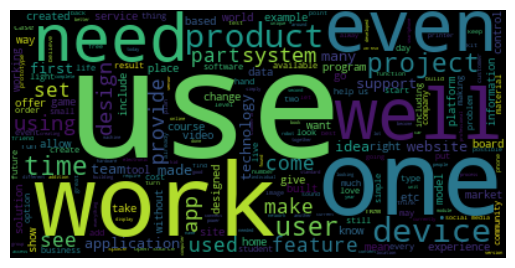
\includegraphics[width=0.7\textwidth]{4/figures/description_wordcloud.png}
		\caption[Nube de palabras de descripciones posterior al pre-procesamiento]{Nube de palabras de descripciones posterior al pre-procesamiento.\\
			Fuente: Elaboración propia.}
		\label{4:fig31}
	\end{center}
\end{figure}

\textbf{Actividad 3: Pre-procesar base de datos de Comentarios}
\\
La base de datos de comentarios está conformada a nivel de 1 proyecto con una lista de comentarios, separados en sublistas y diferenciados entre ellos por autor (patrocinador). De los 7,750 proyectos con comentarios (de los cuales, 4,626 fueron exitosos), se removieron aquellos que presentaron términos en idioma distinto al inglés, así como URLs, emoticonos, emojis, números y caracteres especiales, resultando finalmente en 7,658 proyectos con comentarios (4,574 exitosos).

Debido a la gran cantidad de registros carecientes de comentarios, se propuso rellenarlos con un término aleatorio no relacionado con las temáticas principales: \textit{kuwagatabaizan}. Posteriormente, se repitió el mismo flujograma de la Figura \ref{4:fig30} para las descripciones. Sin considerar este nuevo término, la nube de palabras se representa en la Figura \ref{4:fig32}.

\begin{figure}[!ht]
	\begin{center}
		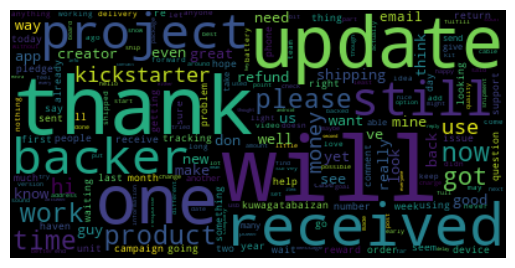
\includegraphics[width=0.7\textwidth]{4/figures/comments_wordcloud_processed.png}
		\caption[Nube de palabras de comentarios posterior al pre-procesamiento]{Nube de palabras de comentarios posterior al pre-procesamiento.\\
			Fuente: Elaboración propia.}
		\label{4:fig32}
	\end{center}
\end{figure}

\section{Modelamiento}
Una vez generadas las variables independientes (observaciones, X) y dependiente (estado de financiamiento, Y), el conjunto de datos es separado en subconjuntos de entrenamiento y prueba, con proporciones de 80\% y 20\% respectivamente (\citeauthor{pr_yuan2016textanalytics}, séptimo antecedente; \citeauthor{pr_yu2018deeplearning}, undécimo antecedente; \citeauthor{pr_chen2019keywords_crowdfunding}, decimoquinto antecedente; \citeauthor{pr_mitra2014phrases}, segundo antecedente; \citeauthor{pr_sawhney2016usingLT}, octavo antecedente) y se fija un valor de aleatoriedad. Dentro de los parámetros de separación, se establece el argumento de estratificación según la variable Y dentro de la función \textit{train\_test\_split}, de la siguiente manera:

\begin{lstlisting}[language=Python]
train_test_split(X, Y, test_size = 0.20, stratify = Y, random_state=0)
\end{lstlisting}

Antes de crear los modelos correspondientes, y después de definir los valores de entrada y parámetros (las subsecciones que se detallarán a continuación), se asigna una semilla inicial con un valor fijado por el usuario con el fin de evitar resultados aleatorios para futuras iteraciones. Se establece, además, una ruta local en donde se almacena cada punto de control basado en la mejora de la pérdida del subconjunto de validación con respecto a su iteración anterior. En caso de un estancamiento de esta última durante 10 épocas, es decir, si el valor de la pérdida no decrementa, el modelo dejará de entrenar. A esta regla se le añade la reducción de la tasa de aprendizaje luego de 5 épocas en caso el valor de la exactitud del subconjunto de validación no refleje un incremento. El objetivo de estas condiciones es evitar el sobreajuste en los modelos.

Por último, es importante asignar un peso distinto para cada una de las dos clases de la variable dependiente \textit{state}. Con el fin de evitar un mal entrenamiento, los pesos de ambas clases se balancean y se almacenan en un diccionario con su etiqueta correspondiente.

\textbf{Actividad 1: Desarrollar modelo predictivo de Metainformación}
\\
Se diseñó el modelo de descripciones basada en un Perceptrón Multicapa (MLP por sus siglas en inglés) bajo la arquitectura de la Figura \ref{4:fig33} y teniendo como referencia a los autores \citeauthor{pr_yu2018deeplearning} (undécimo antecedente). Se asignaron 100 épocas y el número de lotes fue 32.

\begin{figure}[!ht]
	\begin{center}
		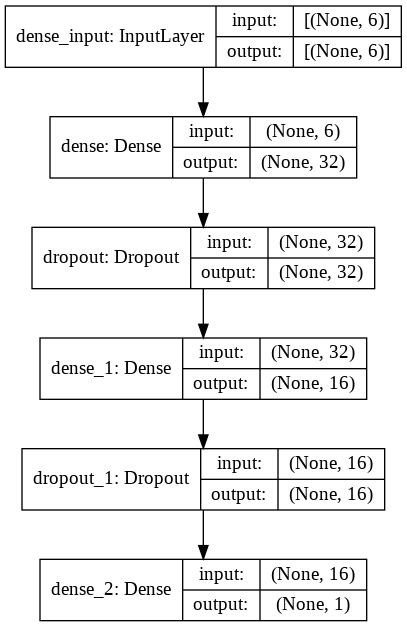
\includegraphics[width=0.40\textwidth]{4/figures/model_mlp_metadata.png}
		\caption[Arquitectura de modelo MLP para la metadata]{Arquitectura de modelo MLP para la metadata.\\
			Fuente: Elaboración propia.}
		\label{4:fig33}
	\end{center}
\end{figure}

La arquitectura comienza con la capa de entrada alimentadas por las 6 variables consideradas, la cual asimismo representará la cantidad de neuronas, tanto de entrada como de salida.

Si bien no existe alguna regla general para definir el número de capas óptimas, así como los hiperparámetros que se deben configurar en ellas, se puede utilizar como referencia algunas metodologías como las Reglas del Pulgar \parencite{tec_ranjan2019thumbrules}.

De acuerdo a algunas de estas, el número de capas ocultas comienza con 2 sin contar la última. La primera capa densa continúa a la capa de entrada, mientras que la segunda aparece después de la primera capa de desactivación.

Otro punto considerado fue el número de nodos o neuronas de las capas intermedias. Estas deben seguir una progresión geométrica de 2, donde la primera capa debe ser la mitad del número de variables en la capa de entrada. Dado que la mitad de 6 es un valor que no cumple, un número potencial puede ser 4.

El autor de algunas de estas reglas también menciona tener en consideración utilizar la función de activación \textbf{relu} para las capas intermedias, una tasa de abandono de por lo menos 0.5 para las capas de desactivación, tamaño de salida de 1 neurona y función de activación \textbf{sigmoide} por tratarse de un problema de clasificación binaria, utilizar el optimizador \textbf{adam}, comenzar con 20 épocas en adelante de acuerdo al progreso de los resultados y fijar un tamaño de lote bajo progresión geométrica de 2; además de otros requerimientos previamente establecidos como la ponderación de clases para la variable dependiente en caso de datos desbalanceados y escalado de datos antes del entrenamiento.

Todas estas opciones fueron probadas en el modelo y evaluadas con las métricas correspondientes. Sin embargo, al calibrar el modelo y comparar distintos resultados, se obtuvo que la mejor cantidad de neuronas para la primera capa densa era de 32. De este modo, la siguiente capa intermedia se le asignó la mitad (16). La función de activación \textbf{tanh} para la segunda capa oculta presentó mejores resultados, así como tasas de abandono entre 0.25 y 0.3 para las capas de desactivación. Por último, además de \textit{adam}, se realizó experimentos con otros optimizadores como por ejemplo \textit{RMSprop} siendo este el resultado más cercano. Al final, \textit{adam} fue escogido pero con una tasa de aprendizaje baja como 0.005 debido a que el modelo tendía a aprender muy rápido durante el transcurso de las épocas. En conjunto, el ratio de decaimiento se asignó un valor más bajo, 0.00005, y para evaluar los subconjuntos de entrenamiento y prueba se eligió precisión como métrica.

\textbf{Actividad 2: Desarrollar modelo predictivo de Descripción}
\\
Para crear la capa de incrustación de palabras, se usó la función \textit{Tokenizer} de la librería \textbf{tensorflow.keras.preprocessing.text}, creando una función para originar un diccionario de palabras a índice al subconjunto de entrenamiento, asignándose a cada una un código. La función creada asimismo permite colocar un valor (en este caso, el término \textit{$<$OOV$>$}) a aquellos términos no entrenados y serán parte de la data de prueba (Figura \ref{4:fig34}). A continuación, los arreglos de estos textos codificados son rellenados con ceros a la derecha, hasta uniformizar con la longitud de la descripción más larga, ya que todas presentan distintos tamaños (Figura \ref{4:fig35}).

\begin{figure}[htbp]
	\begin{center}
		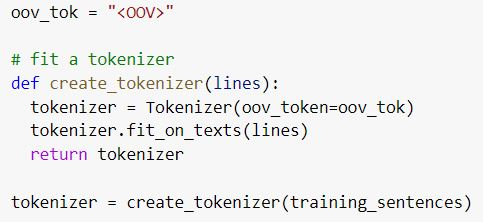
\includegraphics[width=0.50\textwidth]{4/figures/description_tokenizer_function.jpg}
		\caption[Función de tokenización de palabras de descripciones]{Función de tokenización de palabras de descripciones.\\
			Fuente: Elaboración propia.}
		\label{4:fig34}
		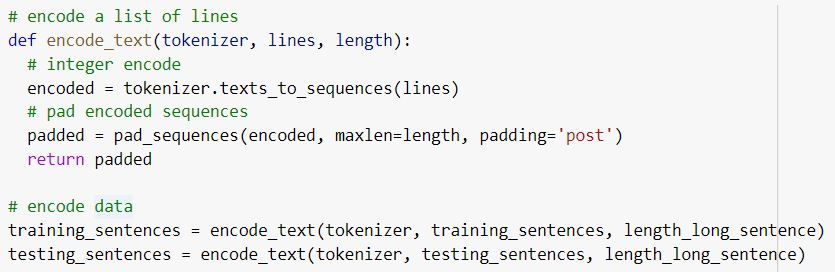
\includegraphics[width=0.80\textwidth]{4/figures/description_encoder_function.jpg}
		\caption[Función de codificación de palabras y rellenado de arreglos]{Función de codificación de palabras y rellenado de arreglos.\\
			Fuente: Elaboración propia.}
		\label{4:fig35}
	\end{center}
\end{figure}

Una vez obtenido el vocabulario de palabras únicas y asignado el tamaño de cada arreglo (en este caso, se asignó el de la descripción de mayor longitud), se procedió a elaborar la matriz de características usando incrustaciones de GloVe (Figura \ref{4:fig36}). Para la presente investigación, se seleccionó la opción Wikipedia 2014 + Gigaword 5, con una matriz de 100 columnas, donde cada una contendrá las incrustaciones de palabras GloVe para las palabras del corpus, cuyos índices se corresponderán con cada número de fila \parencite{tec_malik2019pythonnlp}.

\begin{figure}[!ht]
	\begin{center}
		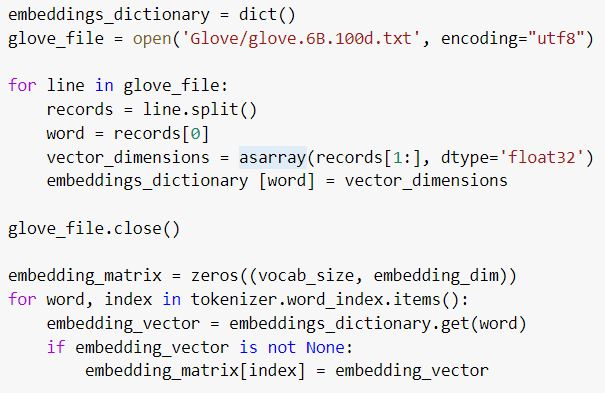
\includegraphics[width=0.55\textwidth]{4/figures/description_glove.jpg}
		\caption[Elaboración de matriz de incrustaciones de palabras]{Elaboración de matriz de incrustaciones de palabras.\\
			Fuente: Elaboración propia.}
		\label{4:fig36}
	\end{center}
\end{figure}

Se diseñó el modelo de descripciones basada en una Red Neuronal Convolucional bajo la arquitectura de la Figura \ref{4:fig37}, así como de referencia un trabajo de análisis de sentimientos de películas \parencite{tec_malik2019pythonnlp}. Se asignaron 100 épocas para entrenar y número de lotes de 128.

\begin{figure}[!ht]
	\begin{center}
		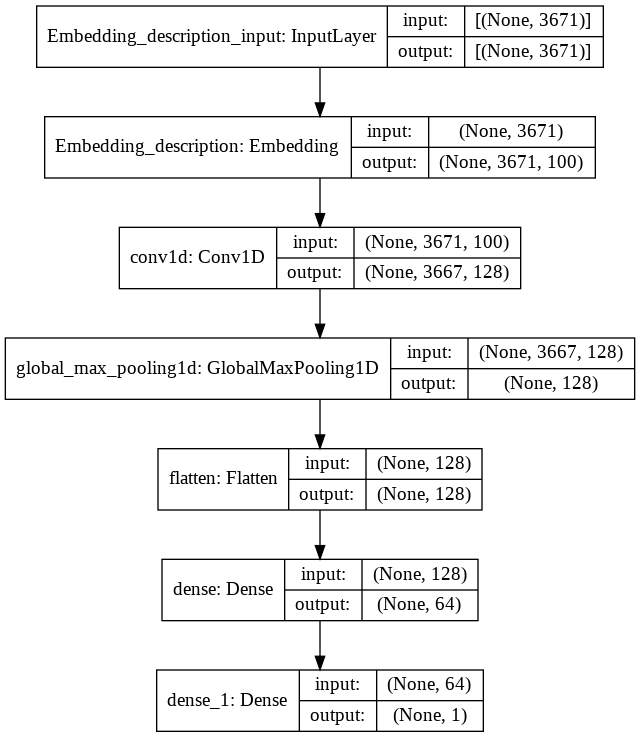
\includegraphics[width=0.60\textwidth]{4/figures/model_cnn_description.png}
		\caption[Arquitectura de modelo CNN para las descripciones]{Arquitectura de modelo CNN para las descripciones.\\
			Fuente: Elaboración propia.}
		\label{4:fig37}
	\end{center}
\end{figure}

Esta red se compone de una capa de incrustación de palabras o \textit{Embedding} alimentada por los datos de entrada en la primera capa \textit{InputLayer} de dimensión de 3,671 vectores de palabras (la mayor longitud de palabras de todas las descripciones), la cual genera como salida una matriz de 3,671 por 100 (número de columnas de incrustaciones de GloVe). Para esta capa se entrenarán 14,827,000 parámetros como resultado del producto de las 100 columnas mencionadas y 148,270 como el tamaño del vocabulario entrenado.

La siguiente capa es la Convolución en 1 dimensión o \textit{Conv1D} (usado frecuentemente para extraer características de datos de textos por ser unidimensionales) que, con 128 características, 5 de tamaño de kernel y función de activación \textbf{relu}, generó una salida de 3,667 por 128; así como 64,128 parámetros entrenables.

A continuación, le sigue la capa de reducción \textit{GlobalMaxPooling}. Al igual que en la convolución, esta también fue unidimensional y se caracteriza por realizar agrupamiento global basado en el valor máximo de los bloques seleccionados para reducir el tamaño del vector.

Esta nueva salida pasa por la capa de aplanamiento o \textit{Flatten}, en donde se multiplican las filas y columnas y tener un solo vector. Esta sirve para conectar con las 64 neuronas de la nueva capa densa y función de activación \textbf{tanh}, agregada con el fin de mejorar la performance del modelo. El criterio para considerar una función \textit{tanh} obedece al mejor desempeño durante el entrenamiento que la función \textit{relu}, evitando el sobreajuste durante mayores épocas ocasionado por gradientes que desaparecen al propagar hacia atrás a mayor cantidad de capas. El uso de la función tangente hiperbólica en capas ocultas resultó una buena práctica durante las décadas de 1990 y 2000, teniendo mejor rendimiento que la función logística \parencite{tec_brownlee2019vanishing_gradients}. Aún así, ambas son dos opciones válidas para problemas de redes neuronales profundas.

Finalmente, la arquitectura culmina con la última capa con función de activación \textbf{sigmoid} para regular el valor de salida entre 0 y 1, ya que se trata de un problema de clasificación binaria (por ello, también cuenta con solo 1 neurona y su parámetro de pérdida es “\textit{binary\_crossentropy}”).

\textbf{Actividad 3: Desarrollar modelo predictivo de Comentarios}
\\
Al igual que en el modelo de descripciones de proyectos, se creó un diccionario de palabras con la data luego de tokenizar y codificarlas con las mismas funciones y librerías. Sin embargo, a diferencia del anterior modelo, la longitud de la matriz para el rellenado de ceros con el fin de homogenizar el tamaño de cada vector de incrustaciones se limitó a las 5,000 últimas palabras de una oración (parámetro \textbf{padding='post'} de la función \textit{pad\_sequences}) en lugar de la longitud máxima dado que ésta representa una cantidad considerable (30,072) como para utilizar todos los recursos del entorno de ejecución.

De igual manera, se creó una matriz de incrustaciones de palabras usando GloVe y se diseñó una arquitectura basada en una Red Neuronal Recurrente (RNN por sus siglas en inglés) ilustrada en la Figura \ref{4:fig38}.

\begin{figure}[!ht]
	\begin{center}
		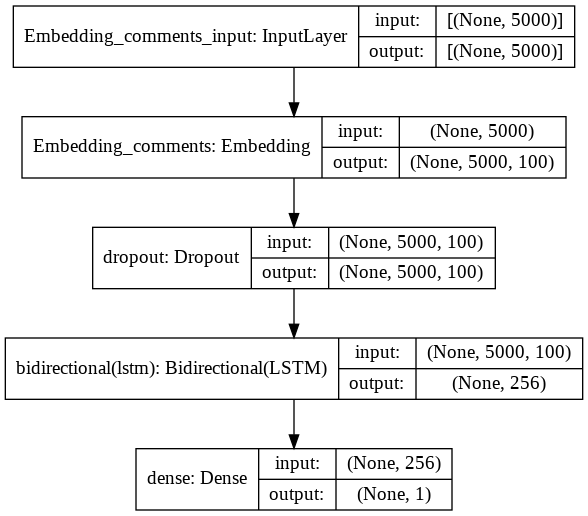
\includegraphics[width=0.60\textwidth]{4/figures/model_rnn_comments.png}
		\caption[Arquitectura de modelo RNN para los comentarios]{Arquitectura de modelo RNN para los comentarios.\\
			Fuente: Elaboración propia.}
		\label{4:fig38}
	\end{center}
\end{figure}

Existe una similitud de estructura en las 2 primeras capas con las del modelo de descripción. Luego de la capa de incrustaciones o \textit{Embedding}, para reducir las conexiones entre neuronas se añadió 1 capa de desactivación o \textit{Dropout}.

A continuación, los vectores de palabras ingresan a la capa de la red neuronal recurrente \textit{LSTM}. Para este caso, se consideró envolverla dentro de una Red Bidireccional de 128 neuronas, ya que como se explicó en el Marco Teórico del Capítulo II sobre las RNN Bidireccionales, este tipo es una mejora de la LSTM tradicional al entrenar 2 juntas (la segunda representa una copia invertida de la secuencia de entrada) en donde cada capa ahora puede considerar también información de las capas siguientes junto con la información de las previas que ya tenía en cuenta, es decir, toma información de 2 direcciones \parencite{tec_brownlee2017bidirectional_lstm}.

Finalmente, el modelo culmina con una capa densa en donde recibe 256 valores de entrada (2*128 de la capa Bidireccional LSTM) y utiliza la función de activación \textit{sigmoid} para transformar el valor final entre 0 y 1.

En la Tabla \ref{4:table3} se presentan las variables que se usaron para entrenar el modelo de Aprendizaje Profundo Multimodal. Estas fueron seleccionadas de acuerdo al Benchmarking aplicado a los 17 antecedentes en el Capítulo II.

\begin{table}[h!]
	\caption[Diccionario de datos del conjunto final entrenado]{Diccionario de datos del conjunto final entrenado.}
	\label{4:table3}
	\centering
	\small
	\begin{tabular}{ |m{3cm}|m{10cm}|m{2cm}|  }
		\hline
		%\rowcolor{bluejean}
		\Centering \textbf{Variable}& \Centering \textbf{Detalle}& \Centering \textbf{Tipo de dato}\\
		\hline
		%\rowcolor{turq}
		\multicolumn{3}{c}{Variables independientes} \\
		\hline
		\textbf{goal} &	Monto de la meta de financiamiento del proyecto. &	float64 \\
		\hline
		\textbf{completeness} & Porcentaje de financiamiento o completitud. & float64 \\
		\hline
		\textbf{duration} &	Duración de la campaña (en días). &	int64 \\
		\hline
		\textbf{pledges\_num} &	Cantidad de montos disponibles para contribuir. &	int64 \\
		\hline
		\textbf{pledged} &	Monto contribuído en la campaña. &	float64 \\
		\hline
		\textbf{pledges\_median} &	Mediana de montos disponibles para contribuir. &	float64 \\
		\hline
		\textbf{description} &	Descripción del proyecto. &	object \\
		\hline
		\textbf{comments} & Comentarios de patrocinadores sobre el proyecto. & object \\
		\hline
		%\rowcolor{turq}
		\multicolumn{3}{c}{Variable dependiente} \\
		\hline
		\textbf{state} & Estado de financiamiento del proyecto. & object \\
		\hline
	\end{tabular}
	\par	%%Salto de linea
	\bigskip
	\begin{flushleft}	%%Alinear a la izquierda sin justificar
		\small Fuente: Elaboración propia.
	\end{flushleft}
\end{table}

Los autores citados por cada variable utilizada se mencionan a continuación:
\begin{itemize}
	\item \textbf{goal}: \cite{pr_chen2013kickpredict}, \cite{pr_mitra2014phrases}, \cite{pr_zhou2015projectdesc}, \cite{pr_chen2015predcrowd}, \cite{pr_li2016predcrowd}, \cite{pr_yuan2016textanalytics}, \cite{pr_sawhney2016usingLT}, \cite{pr_kaur2017socmedcrowd}, \cite{pr_kamath2018suplearn}, \cite{pr_yu2018deeplearning}, \cite{pr_jin2019dayssuccess}, \cite{pr_cheng2019deeplearning}.
	\item \textbf{completeness}: \cite{pr_chen2015predcrowd}.
	\item \textbf{duration}: \cite{pr_mitra2014phrases}, \cite{pr_zhou2015projectdesc}, \cite{pr_li2016predcrowd}, \cite{pr_sawhney2016usingLT}, \cite{pr_kaur2017socmedcrowd}, \cite{pr_kamath2018suplearn}, \cite{pr_yu2018deeplearning}, \cite{pr_jin2019dayssuccess}.
	\item \textbf{pledges\_num}: \cite{pr_chen2013kickpredict}, \cite{pr_mitra2014phrases}, \cite{pr_chen2015predcrowd}, \cite{pr_yuan2016textanalytics}, \cite{pr_jin2019dayssuccess}.
	\item \textbf{pledged}: \cite{pr_chen2013kickpredict}, \cite{pr_li2016predcrowd}, \cite{pr_kamath2018suplearn}.
	\item \textbf{pledges\_median}: \cite{pr_chen2015predcrowd}*, \cite{pr_jin2019dayssuccess}*.
	\item \textbf{description}: \cite{pr_mitra2014phrases}, \cite{pr_zhou2015projectdesc}, \cite{pr_yuan2016textanalytics}, \cite{pr_sawhney2016usingLT}, \cite{pr_kamath2018suplearn}, \cite{pr_lee2018contentDL}, \cite{pr_jin2019dayssuccess}, \cite{pr_cheng2019deeplearning}, \cite{pr_chen2019keywords_crowdfunding}, \cite{pr_chaichi2019nlp_3dprinting}.
	\item \textbf{comments}: \cite{pr_li2016predcrowd}, \cite{pr_kaur2017socmedcrowd}, \cite{pr_lee2018contentDL}, \cite{pr_jin2019dayssuccess}.
\end{itemize}

Si bien en los respectivos antecedentes marcados en (*) figuran el promedio de los montos disponibles para patrocinar, se usó la mediana en vez de la media ya que presentó mejor performance en los experimentos.

\begin{landscape}
	\textbf{Actividad 4: Desarrollar modelo predictivo ensamblado}
	\\
	Una vez construidos los modelos para cada modalidad (metainformación, descripción y comentarios), se construyó un modelo de Aprendizaje Profundo Multimodal ilustrado en la Figura \ref{4:fig39}.
	
	\begin{figure}[!ht]
		\begin{center}
			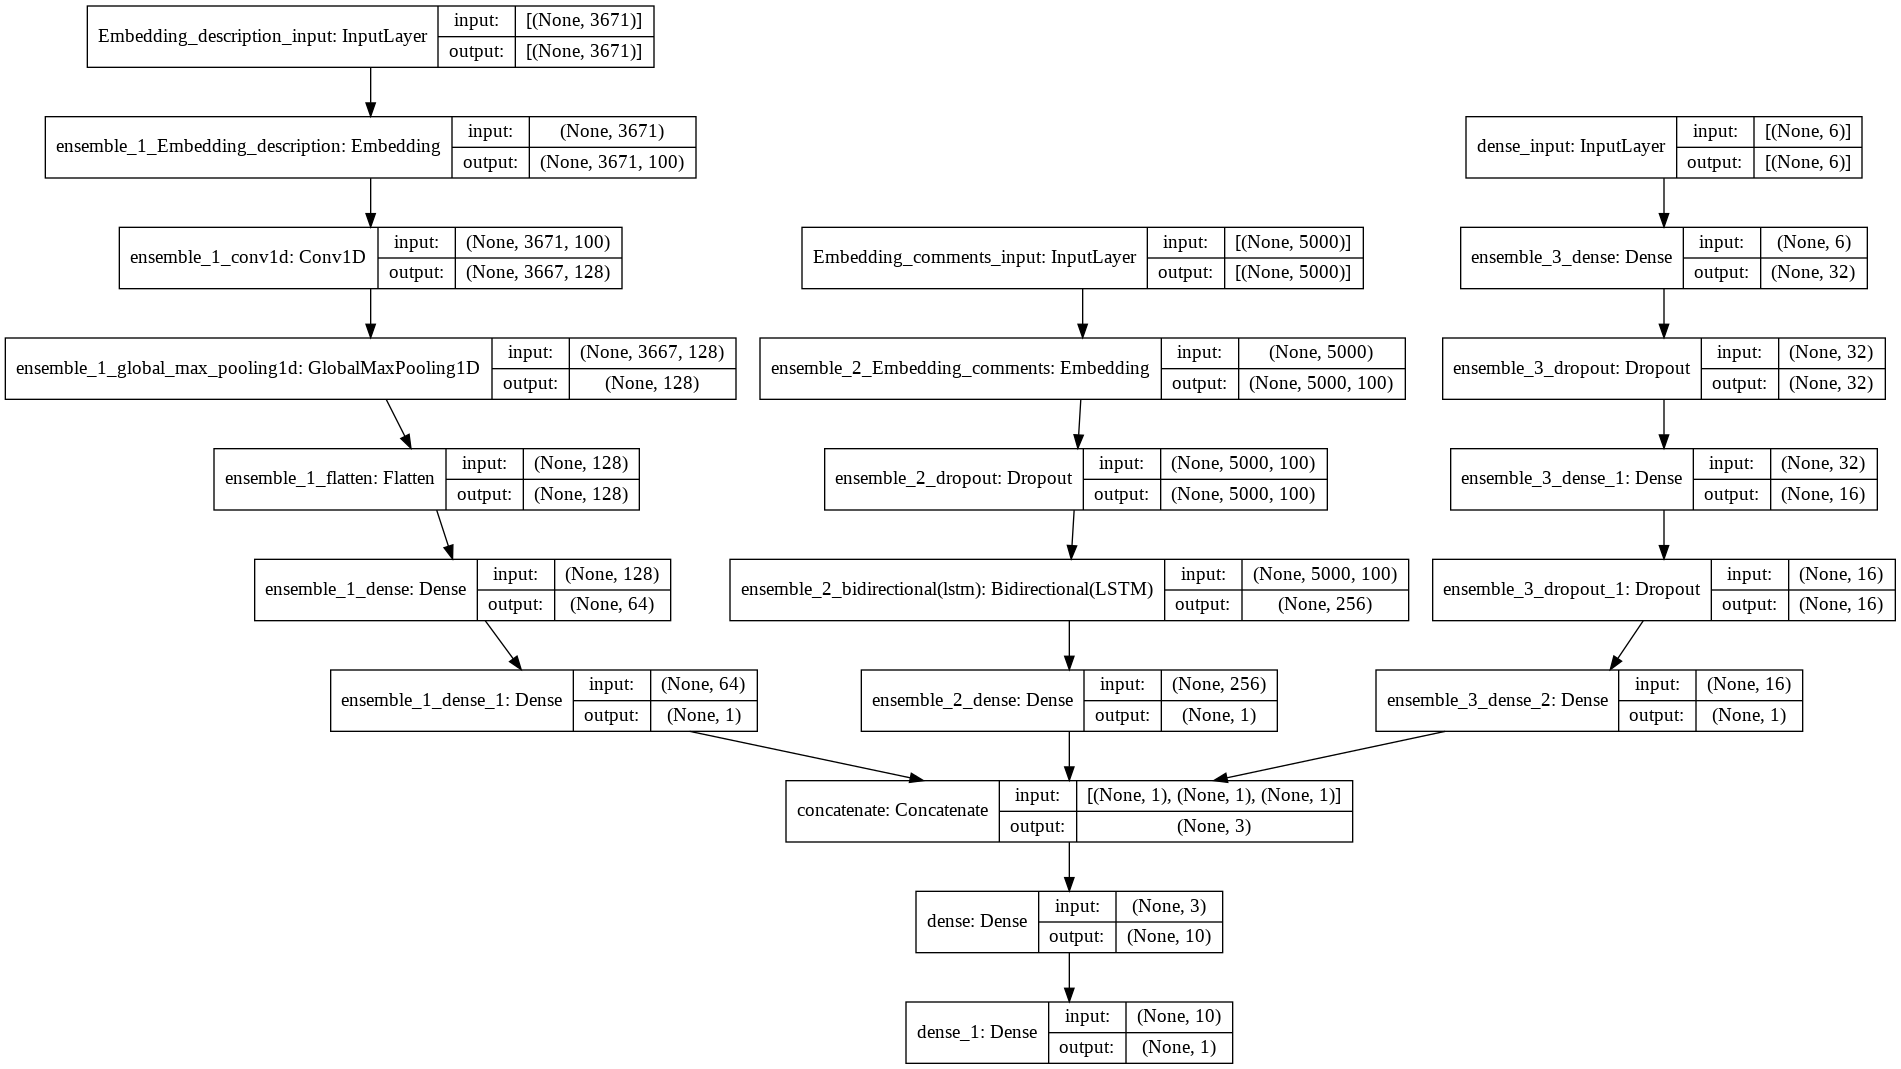
\includegraphics[width=1.20\textwidth]{4/figures/final_stacked_model.png}
			\caption[Arquitectura del modelo apilado final The Hydra]{Arquitectura del modelo apilado final The Hydra.\\
				Fuente: Elaboración propia.}
			\label{4:fig39}
		\end{center}
	\end{figure}
	
\end{landscape}

La finalidad de este modelo apilado de múltiples cabezas es aprender la mejor manera de combinar las predicciones de cada modelo para obtener mejor performance que cada uno individualmente.

A este modelo se le denominó “\textit{The Hydra}” (La Hidra por su traducción al español) en referencia al monstruo mitológico del lago de Lerna, con 7 cabezas que renacían a medida que se cortaban \parencite{ot_rae_hidra}.

Las salidas de cada modelo se concatenaron en una capa debajo de estos, generando 3 valores de entrada para una penúltima capa densa con 10 neuronas de salida y una función de activación ReLu. Finalmente, el modelo apilado culmina con una capa densa de 1 salida y asignándose la función Sigmoide para generar probabilidades entre 0 y 1, los valores de Fracasado o Exitoso respectivamente.

Previo a la compilación del modelo final, se repitió el ejercicio de cada modelo cargado asignar los parámetro de pérdida \textit{binary\_crossentropy} para la clasificación binaria, \textit{accuracy} (exactitud) para la métrica del entrenamiento, pesos balanceados para las clases de la variable \textit{state} (0.6987077585764833 para 0 y 1.7581290322580645 para 1), y optimizador \textit{Adam} con la variante de asignarle el ratio de aprendizaje y también de decaimiento de 0.00005.

\section{Evaluación}

\section{Despliegue}